\documentclass[aspectratio=169
              ,usenames
              ,dvipsnames
              %uncomment to see notes
              %,handout
              ]{beamer}

\usetheme{metropolis}
%gets rid of bottom navigation bars
\definecolor{iicolor}{RGB}{232,150,70}
\setbeamercolor{frametitle}{bg=iicolor}
%\setbeamercolor{frametitle}{bg=white, fg=black}

\setbeamertemplate{footline}[frame number]{}

%gets rid of bottom navigation symbols
\setbeamertemplate{navigation symbols}{}

%gets rid of footer
%will override 'frame number' instruction above
%comment out to revert to previous/default definitions
\setbeamertemplate{footline}{}

%un-comment to see the notes
%\setbeameroption{show only notes} 

\usepackage{appendixnumberbeamer}
\usepackage{mathtools}
\usepackage{environ}
\usepackage{booktabs}
\usepackage{xcolor}
\usepackage{graphicx}
\usepackage{subcaption}
\captionsetup{compatibility=false}
\usepackage[scale=2]{ccicons}
\usepackage{hyperref}
\usepackage{pgfplots, pgfplotstable}
\usepackage{xparse}
\usepgfplotslibrary{dateplot}
\pgfplotsset{compat=1.12} % for better axis label placement

% Create a function for generating inverse normally distributed numbers using the Box–Muller transform
\pgfmathdeclarefunction{invgauss}{2}{%
  \pgfmathparse{sqrt(-2*ln(#1))*cos(deg(2*pi*#2))}%
}

\pgfmathsetseed{3}
% Initialise an empty table with a certain number of rows
\pgfplotstablenew[
    create on use/x/.style={create col/expr=\pgfplotstablerow},
    create on use/brown1/.style={
        create col/expr accum={
            (
                max(
                    min(
                        invgauss(rnd,rnd)*0.1+\pgfmathaccuma,
                        inf % Set upper limit here
                    ),
                    -inf % Set lower limit here
                )
            )
        }{0}
    },
    create on use/brown2/.style={
        create col/expr accum={
            (
                max(
                    min(
                        invgauss(rnd,rnd)*0.1+\pgfmathaccuma,
                        inf
                    ),
                    -inf
                )
            )
        }{0}
    },
    columns={x, brown1, brown2}]{201}\loadedtable 

\usetikzlibrary{decorations.text,graphs,graphs.standard,fadings,shapes.arrows,shadows}

\definecolor{mygray}{RGB}{208,208,208}
\definecolor{background}{RGB}{29,47,43}
\newcommand*{\mytextstyle}{\sffamily\small\bfseries\color{black!85}}
\newcommand{\arcarrow}[3]{%
   % inner radius, middle radius, outer radius, start angle,
   % end angle, tip protusion angle, options, text
   \pgfmathsetmacro{\rin}{2.3}
   \pgfmathsetmacro{\rmid}{2.8}
   \pgfmathsetmacro{\rout}{3.3}
   \pgfmathsetmacro{\astart}{#1}
   \pgfmathsetmacro{\aend}{#2}
   \pgfmathsetmacro{\atip}{5}
   \fill[mygray, very thick] (\astart+\atip:\rin)
                         arc (\astart+\atip:\aend:\rin)
      -- (\aend-\atip:\rmid)
      -- (\aend:\rout)   arc (\aend:\astart+\atip:\rout)
      -- (\astart:\rmid) -- cycle;
   \path[
      decoration = {
         text along path,
         text = {|\mytextstyle|#3},
         text align = {align = center},
         raise = -1.0ex
      },
      decorate
   ](\astart+\atip:\rmid) arc (\astart+\atip:\aend+\atip:\rmid);
}

\usepackage{xspace}
\newcommand{\themename}{\textbf{\textsc{metropolis}}\xspace}
\newcommand\Wider[2][3em]{%
\makebox[\linewidth][c]{%
  \begin{minipage}{\dimexpr\textwidth+#1\relax}
  \raggedright#2
  \end{minipage}%
  }%
}

\title{{\bf Nontraditional Search Engines}}
\date{}
\subtitle{For Fun and (not much) Profit}

\begin{document}

\maketitle
\section{Introduction}
\begingroup
\Huge
\begin{frame}
\frametitle{Introduction}
\begin{center}
Hi, I'm Casey Stella!
\end{center}
\end{frame}
\endgroup

\section{Traditional Search Engines}
\frame{\frametitle{Traditional Approach}
\begin{exampleblock}{}
  {\Large ``In 1911, Professor Lane Cooper published a concordance of William Wordsworth's poetry so that scholars could readily locate words in which they were interested.  The 1,136-page tome lists all 211,000 nontrivial words in the poet's works, from Aaliza to Zutphen's, yet remarkably, it took less than 7 months to construct.  The task was completed so quickly because it was undertaken by a highly organized team of 67 people -- 3 of whom had died by the time the concordance was published -- using 3-by-5 inch cards, scissors, glue, and stamps.''}
  \vskip5mm
  \hspace*\fill{\small--- {\em Managing Gigabytes: Compressing and Indexing Documents and Images} }
\end{exampleblock}
}

\frame{\frametitle{Traditional Approach}
Document Search Engines are really just (sometimes fuzzy) information retrieval systems involving
\begin{itemize}
\item Compressed Document Storage -- Storing the documents in a space-efficient way\pause
\item Indexing -- Intelligently organizing information so that queries can be resolved efficiently and relevant portions of the data extraced quickly.\pause
\item Query Scoring -- Returning relevant needles from the haystack of documents
\end{itemize}
}

\frame{\frametitle{Query Scoring: In the beginning, there was counting}
In order to rank queries, one important aspect is relevance to the query.  Simple ranking systems were constructed around
\begin{itemize}
\item Term Frequency - The number of times a word or query term exists in a document.
\item Document Frequency - The number of documents which contain a query term
\end{itemize}
Together, they can be used to form a numerical statistic that is intended to reflect how important a word is to a document in a collection or corpus.
}

\frame{\frametitle{Query Scoring: Vectors }
Scoring suffered from search engine result inaccuracy due to the vagaries of the human languages.
Synonyms and context which computers lack can make the exercise maddening.
What we needed was a system which could give us more fuzzy matches efficiently.
\begin{itemize}
\item In 2013, Word2Vec was a vectorization model created by Google
\item In 2018, both Google and Facebook released approaches to embed not just words, but also sentences into vectors.
\end{itemize}
{\bf Takeaway:}  With sentences and words embedded into a vector space, query scoring becomes a nearest neighbors search in a vector space
}

\frame{\frametitle{Stellavista!}
A toy search engine, which
\begin{itemize}
\item Index $2.1$M sentences from wikipedia using the released Google Universal Sentence Encoder in Tensorflow
\item Retrieve documents which sentences which are similar to textual queries in ranked order based on textual similarity
\end{itemize}
}

\frame{\frametitle{Stellavista! Architecture}
\begin{center}
  \makebox[\textwidth]{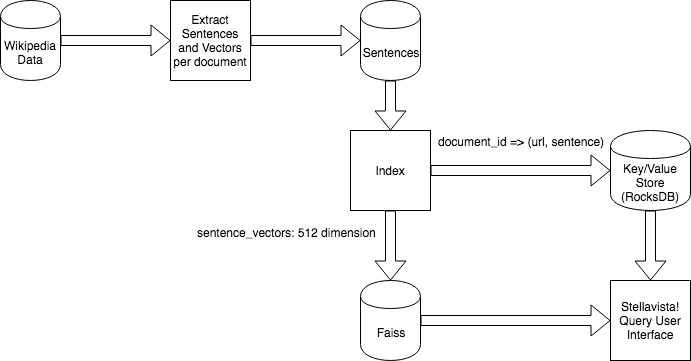
\includegraphics[scale=0.5]{images/architecture.png}}
\end{center}
}

\section{Challenges}

\frame{\frametitle{Sentence Vectorization via Tensorflow}
  A host of lessons were learned:
  \begin{itemize}
    \item The Good\pause
      \begin{itemize}
        \item It was available and (probably) better than just summing or averaging word vectors\pause
        \item Applying a model is embarassingly parallel
      \end{itemize}\pause
    \item The Bad\pause
      \begin{itemize}
      \item Unlike summing or averaging word vectors, it was a lot slower.\pause
      \item Google released a model, not the algorithm, so I can't retrain and add new vocabulary.\pause
      \item There was a massive memory leak which caused me NOT to be able to use Spark for this.
      \end{itemize}
  \end{itemize}
}

\frame{\frametitle{Finding k-Nearest Neighbors in 2M 512-dimensional Vectors Quickly}
  This was a really hard problem, frankly.  After looking around for a comprehensive solution, I landed on a Facebook library called Faiss
  \begin{itemize}
    \item The Good\pause
      \begin{itemize}
        \item Blazing fast\pause
        \item Scales to billions of vectors on a single node\pause
        \item GPU accelerated where appropriate\pause
        \item Supports approximate solutions with latency tradeoffs
      \end{itemize}\pause
    \item The Bad\pause
      \begin{itemize}
      \item Not multi-node parallelizable, but parallelizable via sharding.\pause
      \item Not online updateable.
      \end{itemize}
  \end{itemize}
}

\section{Demo}

\frame{\frametitle{Questions}
Thanks for your attention!  Questions? 
\begin{itemize}
\item Code \& scripts for this talk available on my github presentation page.\footnote{http://github.com/cestella/presentations/}
\item Find me at http://caseystella.com 
\item Twitter handle: @casey\_stella 
\end{itemize}
}

\end{document}
